\documentclass[8pt]{article}
\usepackage{mathrsfs}
\usepackage{amssymb}
\usepackage{amsmath}
\usepackage{amsthm}
\usepackage{mathtools}
\usepackage[pageanchor]{hyperref}
\usepackage{graphicx}
\usepackage{subcaption}
\usepackage{booktabs,siunitx}
\graphicspath{ {./photo/} }

\title{Misura della densità}
\author{Alessandro Rayan Ahmed e Marco Nencioni}

\begin{document}

\maketitle
\pagebreak

\section{Scopo dell'esperienza}
Lo scopo di questa esperienza di laboratorio sta nel calcolare la densità di 13 campioni composti da uno dei 3 material seguentii: alluminio, acciaio inossidabile e ottone.

\section{Cenni teorici}


\begin{displaymath}
	\rho = \frac{m}{V}, \hspace{3mm} [\rho] = kg/m^3
\end{displaymath}

\begin{displaymath}
	V_{\text{sfera}} = \frac{4}{3} \pi r^3
\end{displaymath}

\begin{displaymath}
	V_{\text{parellelepipedo}} = x \cdot y \cdot z
\end{displaymath}

\begin{displaymath}
	\sigma_{V_{\text{sfera}}} = \sqrt{\left(\sigma_{r}\frac{\partial V}{\partial r}\right)^2}
\end{displaymath}

\begin{displaymath}
	\sigma_{V_{\text{parallelepipedo}}} = \sqrt{\left(\sigma_{x}\frac{\partial V}{\partial x}\right)^2 + \left(\sigma_{y}\frac{\partial V}{\partial y}\right)^2 + \left(\sigma_{z}\frac{\partial V}{\partial z}\right)^2}
\end{displaymath}

\pagebreak

\section{Apparato sperimentale}
\paragraph{Strumenti}
\begin{itemize}
\item[1)] Calibro cinquantesimale ($ris.$ 0.02 mm)
\item[2)] Bilancia elettronica ($ris.$ 0.001 g)
\end{itemize}

\paragraph{Materiale}
\begin{itemize}
\item[1)] Cinque sfere di acciaio inossidabile
\item[2)] Due cilindri di ottone e due parallelepipedi di ottone
\item[3)] Due cilindri di alluminio e due parallelepipedi di alluminio
\end{itemize}

\begin{figure}[h!]
  \centering
  \begin{subfigure}[b]{0.3\linewidth}
    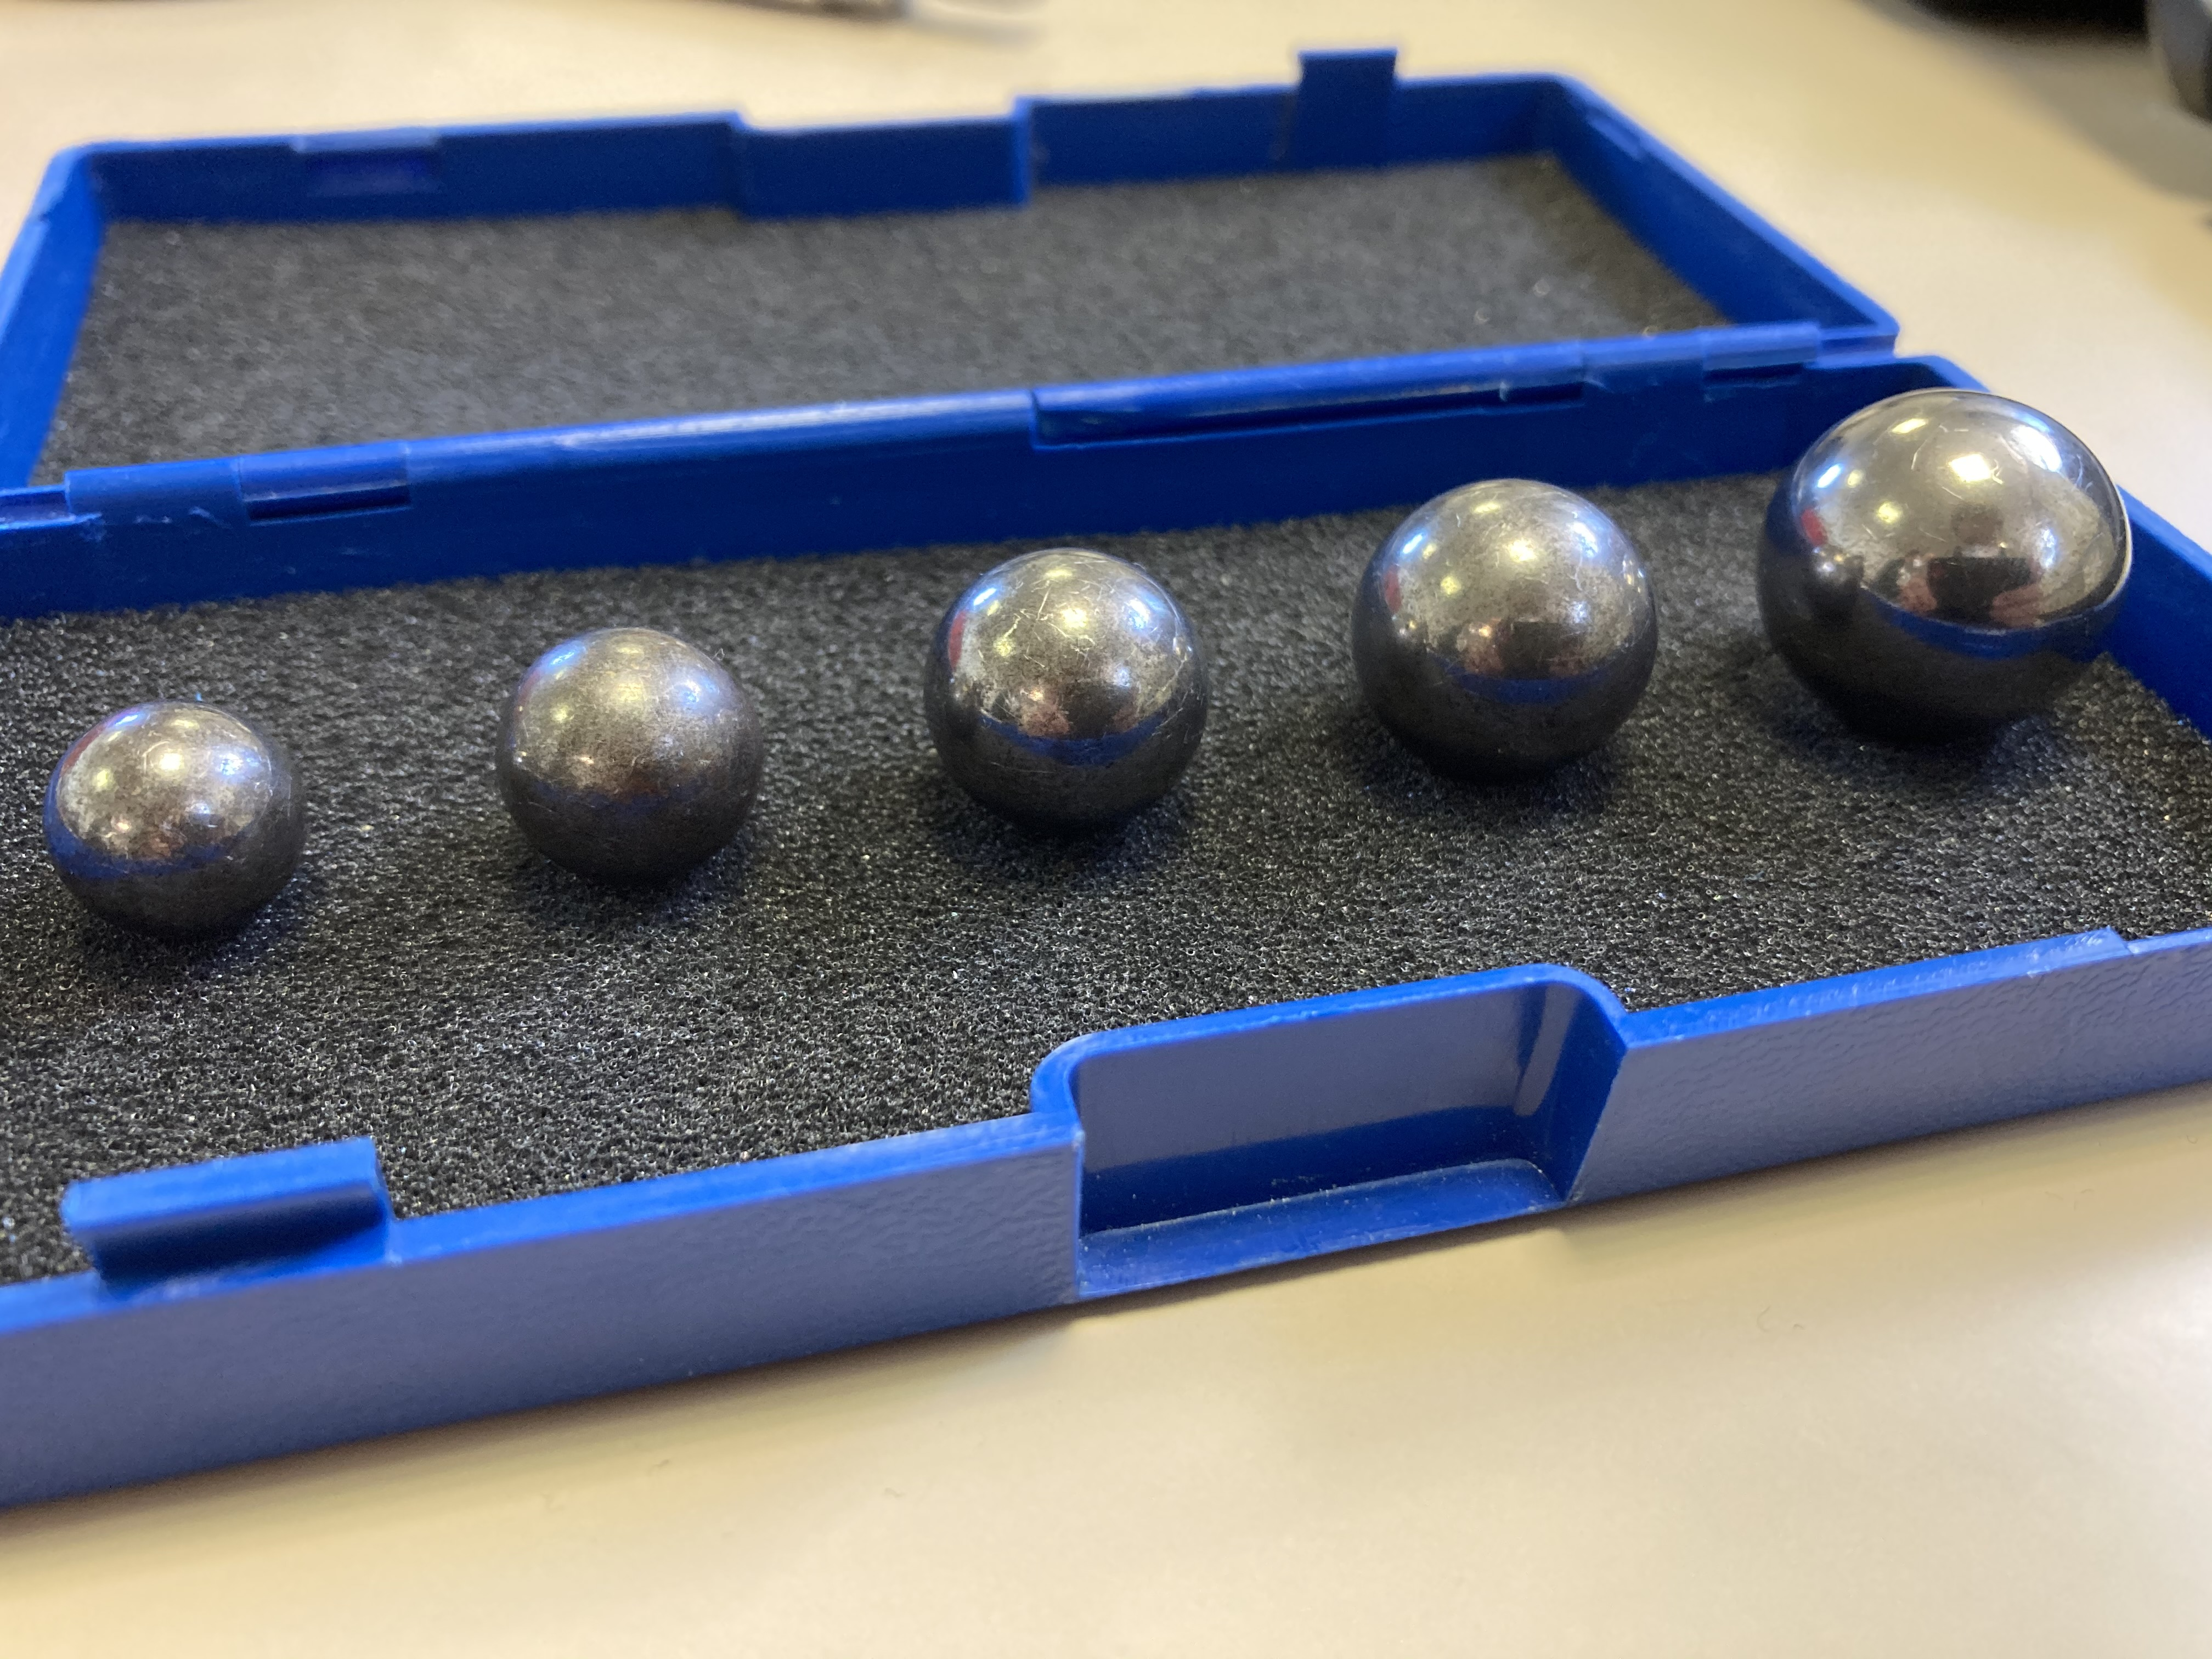
\includegraphics[width=\linewidth]{IMG_6385.jpg}
    \caption{Acciaio.}
  \end{subfigure}
  \begin{subfigure}[b]{0.3\linewidth}
    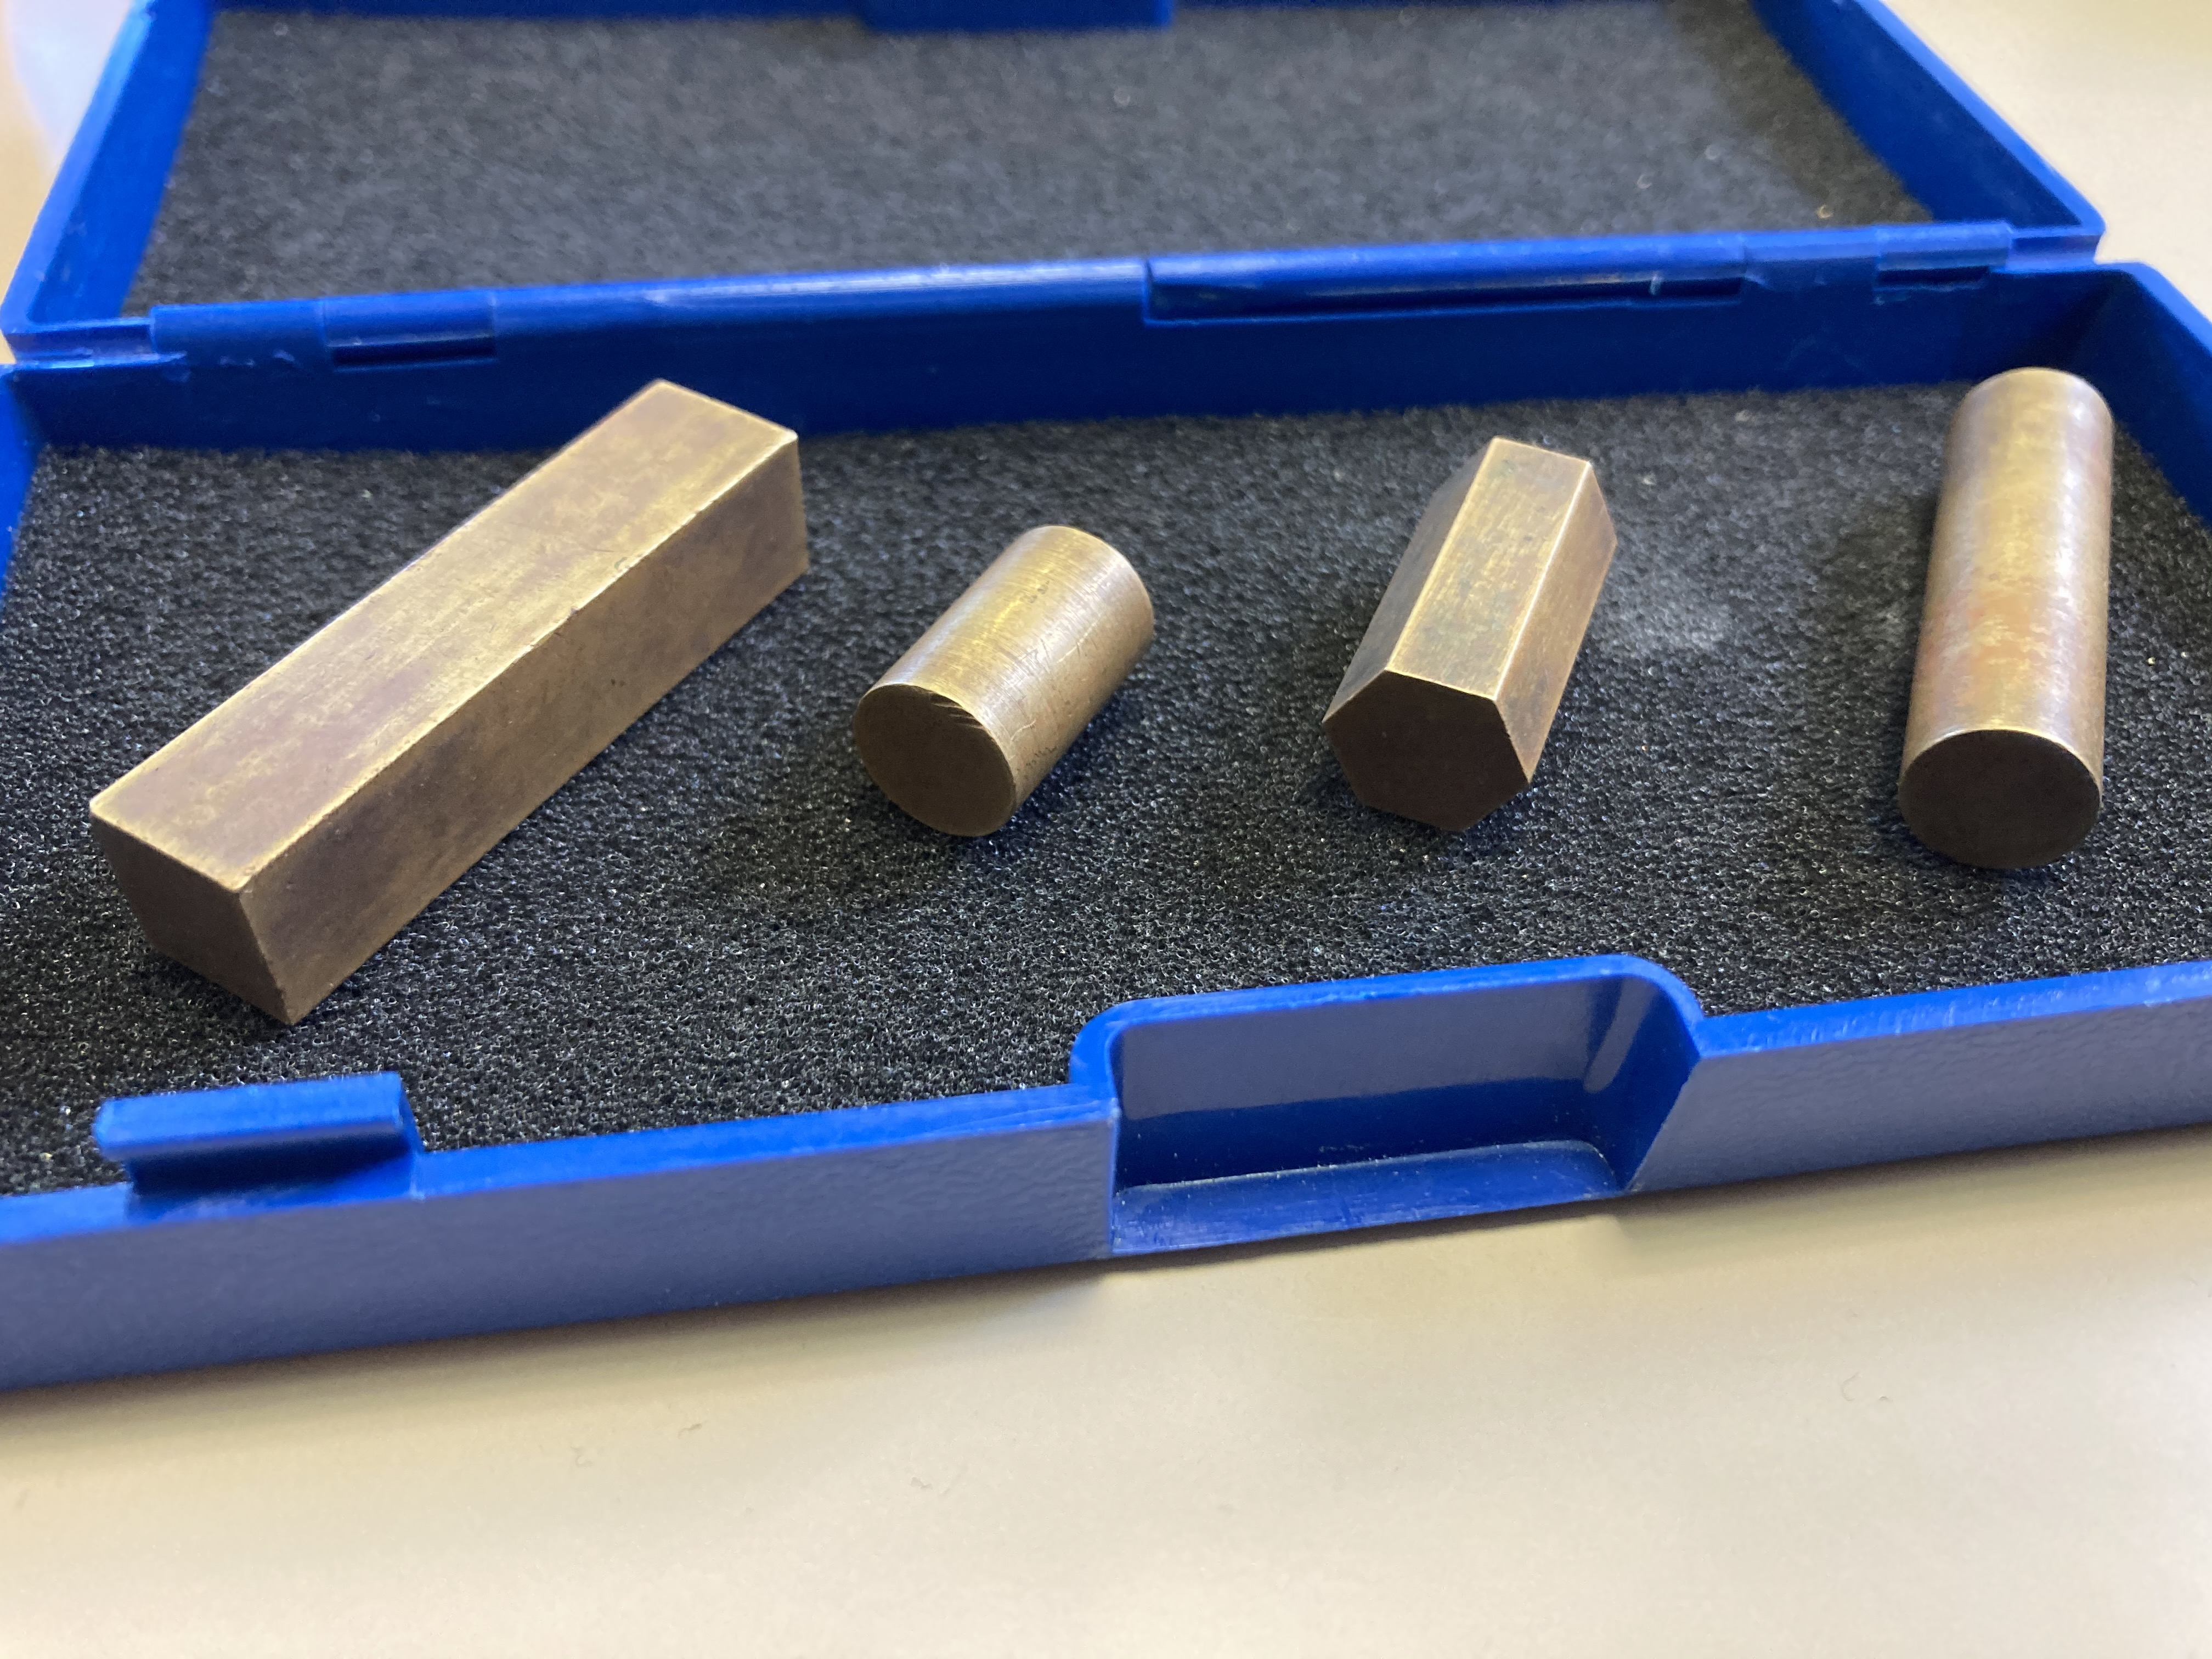
\includegraphics[width=\linewidth]{IMG_6386.jpg}
    \caption{Ottone.}
  \end{subfigure}
\begin{subfigure}[b]{0.3\linewidth}
    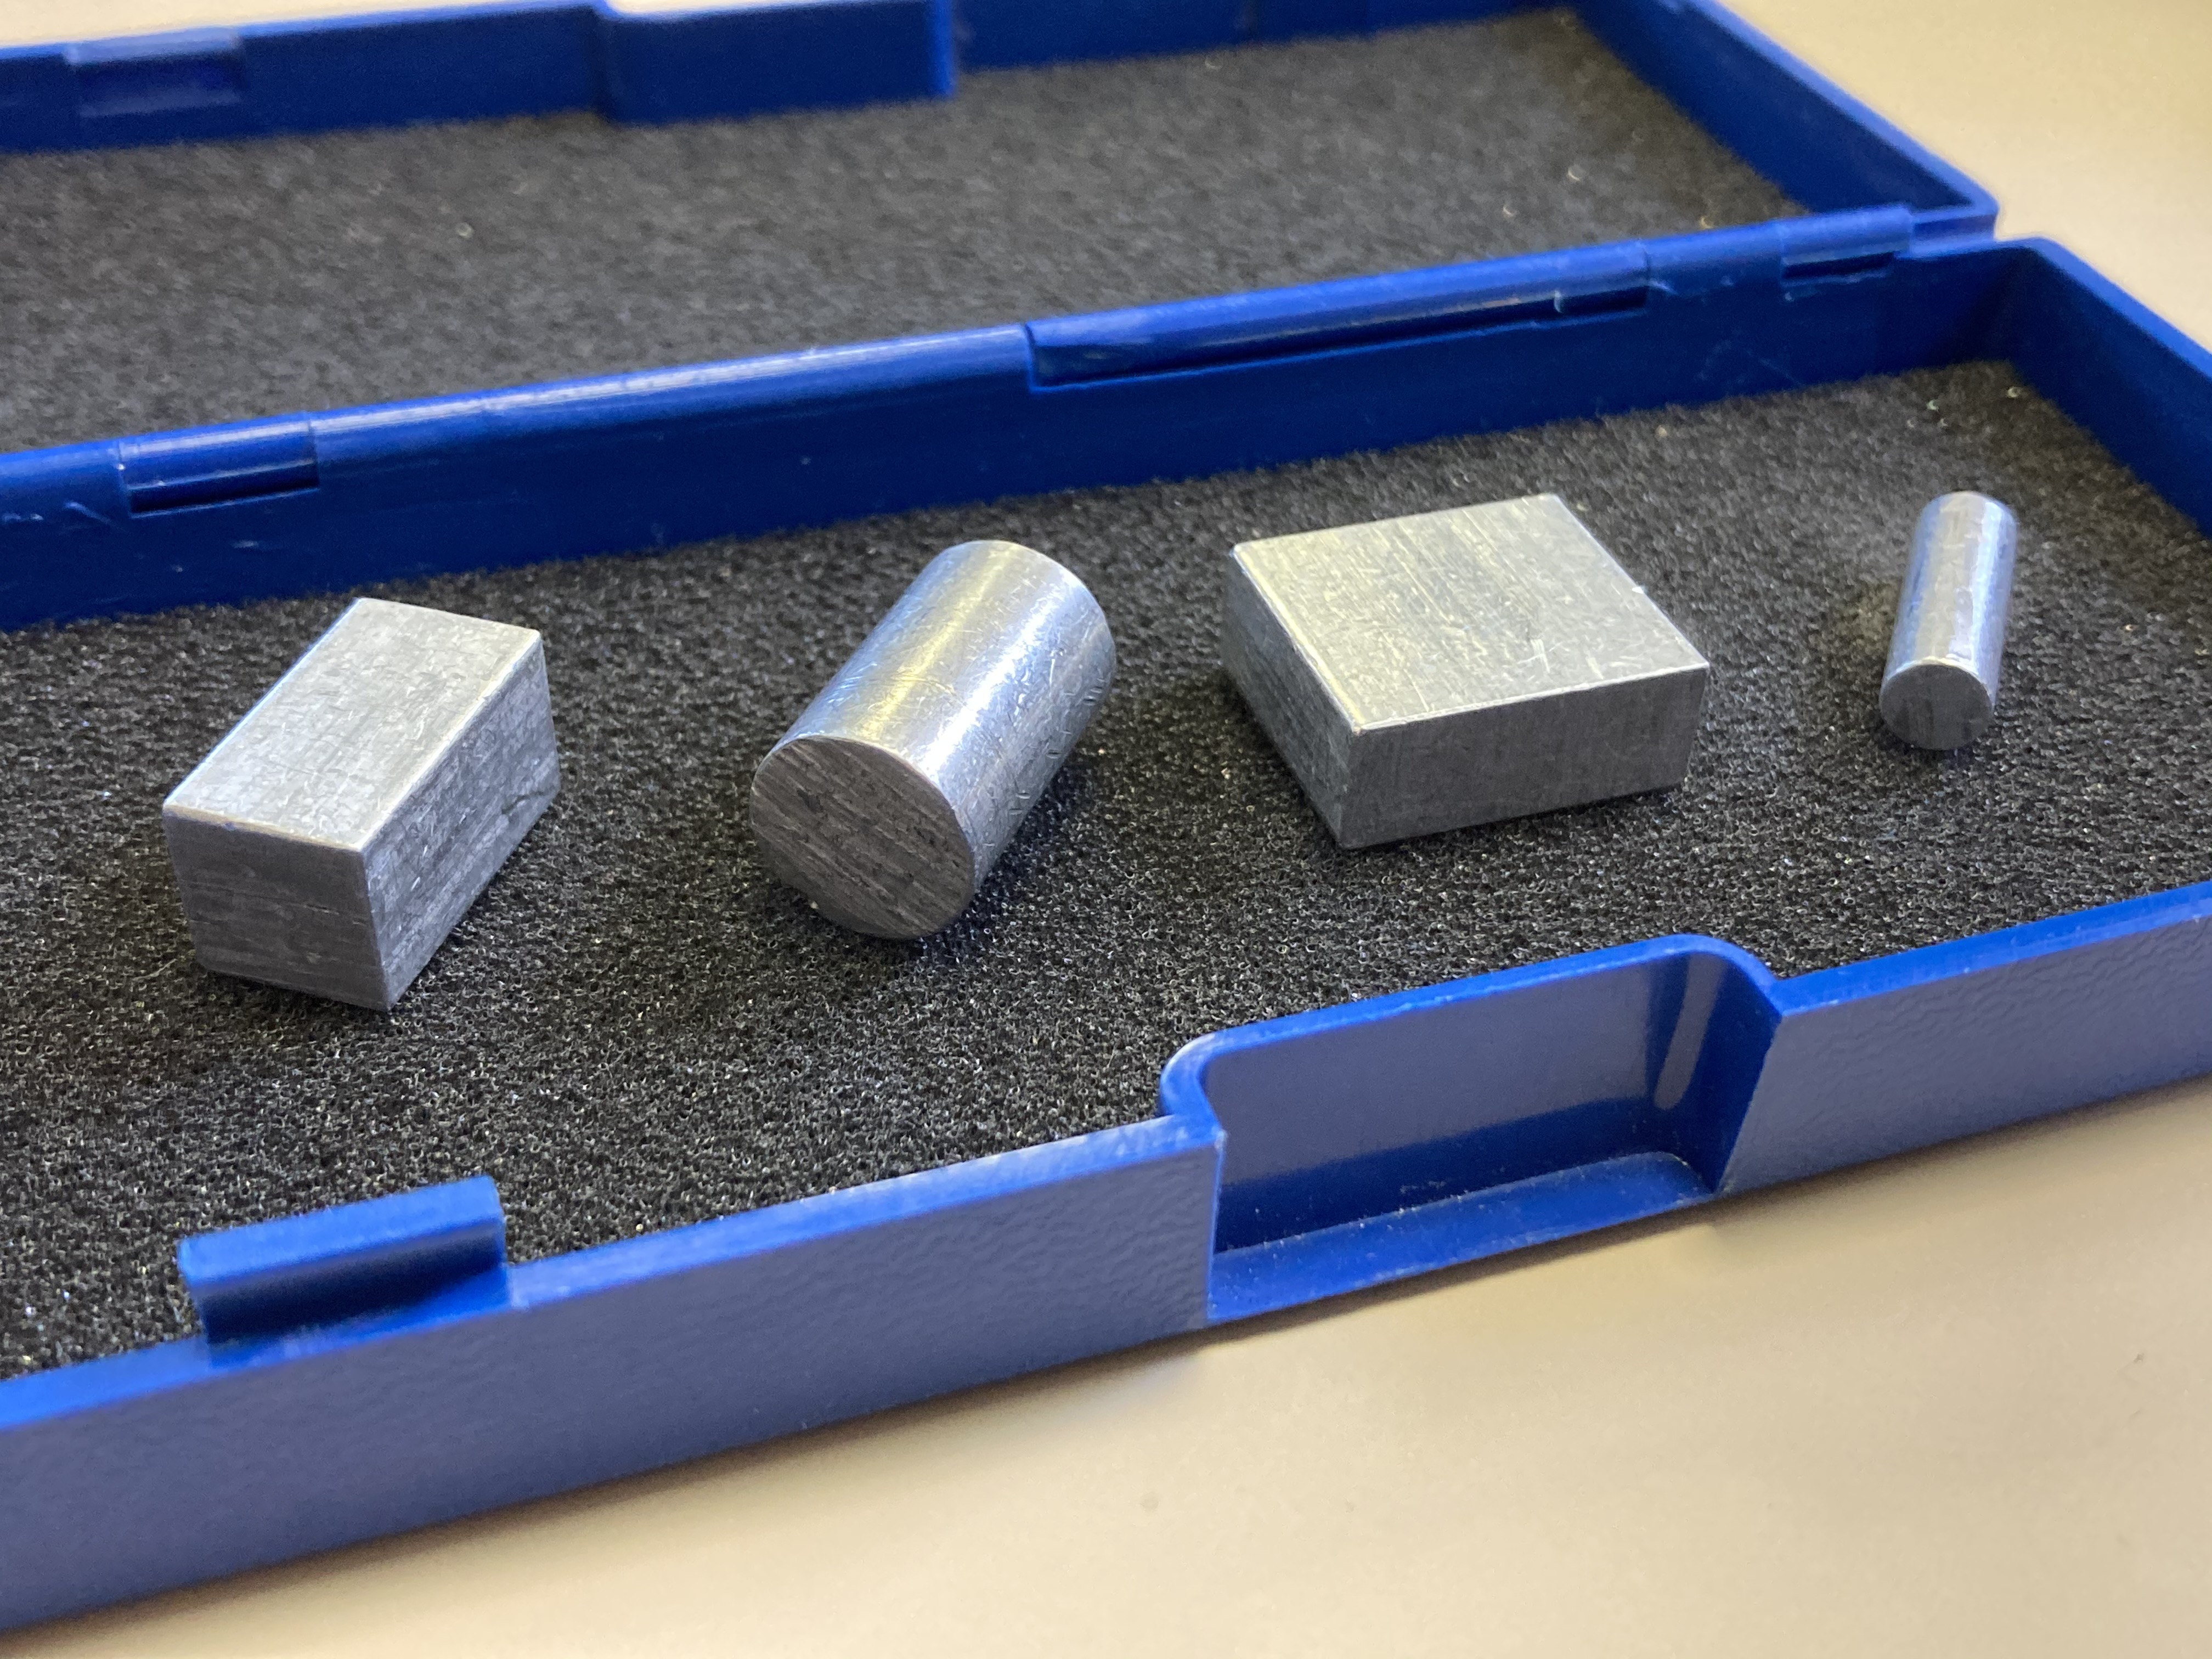
\includegraphics[width=\linewidth]{IMG_6387.jpg}
    \caption{Alluminio.}
  \end{subfigure}
  \caption{I tredici campioni da analizzare sui quali abbiamo calcolato le densità.}
  \label{fig:campioni}
\end{figure}

Il \textbf{calibro cinquantesimale} è uno strumento con la risoluzione di 0.02 mm
impiegato per la misura dei diametri. Esso è stato utilizzato nella misura
delle dimensioni di tutti i campioni. \\

La \textbf{bilancia elettronica} è uno strumento utilizzato per calcolare la massa di un corpo.
In questo caso particolare la nostra bilancia disponeva di una risoluzione di 1 mg.

\section{Descrizione delle misure}
Le misure necessarie per il calcolo dei volumi e delle densità corrispondono alle dimensioni e alle masse
dei campioni. \\
Per calcolare i volumi delle sferette è necessario conoscere il diametro di ogni singola sfera.
Ciò è ottenibile ponendo le tenaglie del calibro sulla circonferenza maggiore della sfera. \\
Mentr  per calcolare i volumi dei parallelepipedi sono è necessario sapere la lunghezza 
(indicata con $x$), la larghezza (indicata con $y$) e l'altezza (indicata con $z$). Per ricavare
tali misure è stato impiegato nuovamente il calibro cinquantesimale, chiudendo le tenaglie su ognuno
dei piani ortogonali del campione. \\

Per misurare le masse dei campioni abbiamo utilizzato la bilancia elettronica disponibile nell'aula
di laboratorio.

\section{Analisi dei dati}
Calcolo dei volumi e densità delle sfere:

\begin{center}
\begin{tabular}{ c c c }
\toprule
$n^o$ sfera & massa [$g$] & diametro sfera [$mm$] \\
\midrule
1 & $8.360 \pm 0.001$ & $12.64 \pm 0.02$ \\
2 & $11.896 \pm 0.001$ & $14.30 \pm 0.02$ \\
3 & $18.914 \pm 0.001$ & $16.64 \pm 0.02$ \\
4 & $24.770 \pm 0.001$ & $18.22 \pm 0.02$ \\
5 & $44.840 \pm 0.001$ & $22.20 \pm 0.02$ \\
\bottomrule
\end{tabular}
\end{center}

\bigskip

\begin{displaymath}
V_{\text{sfera}} = \frac{4}{3} \pi r^3
\end{displaymath}
\begin{displaymath}
\sigma_{V_{\text{sfera}}} = \sqrt{\left(\sigma_{r}\frac{\partial V}{\partial r}\right)^2} \implies \sigma_{r}\frac{\partial V}{\partial r} \implies \sigma_{V_{sfera}} = \sigma_{r} 4 \pi r^2
\end{displaymath}

\smallskip

\begin{center}
\begin{tabular}{ c c c }
\toprule
$n^o$ sfera & volume sfera [$mm^3$] \\
\midrule
1 & $1057 \pm 5$ \\
2 & $1531 \pm 6$ \\
3 & $2412 \pm 9$ \\
4 & $3167 \pm 1 \cdot 10^1$ \\
5 & $5729 \pm 2 \cdot 10^1$ \\
\bottomrule
\end{tabular}
\end{center} 

\bigskip

\begin{displaymath}
\rho_{\text{sfera}} = \frac{m_{\text{sfera}}}{V_{\text{sfera}}}
\end{displaymath}

\smallskip

\begin{center}
\begin{tabular}{ c c c }
\toprule
$n^o$ sfera & densità sfera [$g/mm^3$] \\
\midrule
1 & $7.909 \cdot 10^{-3} \pm 4 \cdot 10^{-5}$ \\
2 & $7.770 \cdot 10^{-3} \pm 3 \cdot 10^{-5}$ \\
3 & $7.842 \cdot 10^{-3} \pm 3 \cdot 10^{-5}$ \\
4 & $7.821 \cdot 10^{-3} \pm 2 \cdot 10^{-5}$ \\
5 & $7.826 \cdot 10^{-3} \pm 3 \cdot 10^{-5}$ \\
\bottomrule
\end{tabular}
\end{center} 

\pagebreak

Calcolo dei volumi e densità dei prismi:

\begin{center}
\begin{tabular}{ c c c c c }
\toprule
$n^o$ prisma & tipo di base & massa [$g$] & diametro base [$mm$] & altezza [$mm$]\\
\midrule
1 & circolare & $10.433 \pm 0.001$ & $10.00 \pm 0.02$ & $16.02 \pm 0.02$ \\
2 & circolare & $24.481 \pm 0.001$ & $10.00 \pm 0.02$ & $37.30 \pm 0.02$\\
3 & esagonale & $16.529 \pm 0.001$ & $10.00 \pm 0.02$ & $22.84 \pm 0.02$ \\
4 & rettangolare & $34.961 \pm 0.001$ & $10.00 \pm 0.02$ & $41.82 \pm 0.02$  \\
5 & circolare & $1.450 \pm 0.001$ & $6.00 \pm 0.02$ & $19.26 \pm 0.02$  \\
6 & circolare & $5.846 \pm 0.001$ & $13.30 \pm 0.02$ & $10.96 \pm 0.02$  \\
7 & rettangolare & $7.769 \pm 0.001$ & $18.92 \pm 0.02$ & $8.10 \pm 0.02$  \\
8 & rettangolare & $4.860 \pm 0.001$ & $10.10 \pm 0.02$ & $18.02 \pm 0.02$  \\
\bottomrule
\end{tabular}
\end{center}

\smallskip

\begin{displaymath}
	V_{\text{parellelepipedo}} = {d_b}^2 \cdot h
\end{displaymath}

\begin{displaymath}
\sigma_{V_{\text{parallelepipedo}}} = \sqrt{\left(\sigma_{d_b}\frac{\partial V}{\partial d_b}\right)^2 + \left(\sigma_{h}\frac{\partial V}{\partial h}\right)^2}
\implies
\end{displaymath}
\begin{displaymath}
\implies \sqrt{\left(\sigma_{d_b}2d_{b}h\right)^2 + \left(\sigma_{h}{d_b}^2\right)^2}
\end{displaymath}

\smallskip

\begin{displaymath}
	V_{\text{cilindro}} = {\left(\frac{d_b}{2}\right)}^2 \cdot \pi \cdot h
\end{displaymath}

\begin{displaymath}
\sigma_{V_{\text{parallelepipedo}}} = \sqrt{\left(\sigma_{d_b}\frac{\partial V}{\partial d_b}\right)^2 + \left(\sigma_{h}\frac{\partial V}{\partial h}\right)^2}
\implies
\end{displaymath}
\begin{displaymath}
\implies \sqrt{\left(\sigma_{d_b}d_{b} \pi h\right)^2 + \left(\sigma_{h}{\left(\frac{d_b}{2}\right)}^2\right)^2}
\end{displaymath}

\smallskip

\begin{displaymath}
	V_{\text{esaprism.}} = 6 \cdot \left(\frac{\frac{d_b}{2} \cdot 2\left(\frac{d_b}{2} \tan(\pi / 6)\right)}{2}\right) \cdot h = 3 \cdot \left(\frac{{d_b}^2 \tan(\pi / 6)}{2}\right) \cdot h = \frac{\sqrt{3}}{2} \cdot {d_b}^2 h
\end{displaymath}

\begin{displaymath}
\sigma_{V_{\text{esaprism.}}} = \sqrt{\left(\sigma_{d_b}\frac{\partial V}{\partial d_b}\right)^2 + \left(\sigma_{h}\frac{\partial V}{\partial h}\right)^2}
\implies
\end{displaymath}
\begin{displaymath}
\implies \sqrt{\left(\sqrt{3} d_b h \sigma_{d_b}\right)^2 + \left(\frac{\sqrt{3}}{2} {d_b}^2 \sigma_{h}\right)^2}
\end{displaymath}

\begin{center}
\begin{tabular}{ c c c c c }
\toprule
$n^o$ prisma & densità\\
\midrule
1 & circolare & $10.433 \pm 0.001$ & $10.00 \pm 0.02$ & $16.02 \pm 0.02$ \\
2 & circolare & $24.481 \pm 0.001$ & $10.00 \pm 0.02$ & $37.30 \pm 0.02$\\
3 & esagonale & $16.529 \pm 0.001$ & $10.00 \pm 0.02$ & $22.84 \pm 0.02$ \\
4 & rettangolare & $34.961 \pm 0.001$ & $10.00 \pm 0.02$ & $41.82 \pm 0.02$  \\
5 & circolare & $1.450 \pm 0.001$ & $6.00 \pm 0.02$ & $19.26 \pm 0.02$  \\
6 & circolare & $5.846 \pm 0.001$ & $13.30 \pm 0.02$ & $10.96 \pm 0.02$  \\
7 & rettangolare & $7.769 \pm 0.001$ & $18.92 \pm 0.02$ & $8.10 \pm 0.02$  \\
8 & rettangolare & $4.860 \pm 0.001$ & $10.10 \pm 0.02$ & $18.02 \pm 0.02$  \\
\bottomrule
\end{tabular}
\end{center}

\pagebreak

\section{Conclusioni}
I risultati dell'esperimento evidenziano le diverse densità dei solidi analizzati, abbiamo constatato che è presente una corrispondenza tra le misure calcolate e i dati a noi proposti. Abbiamo misurato le lunghezze con la precisione del 2\% utilizzando il calibro cinquantesimale e la massa dei solidi con una precisione dell'1\% sfruttando una bilancia elettronica. Per misurare le incertezze relative al volume abbiamo calcolato lo scarto quadratico medio tra le lunghezze mentre relativamente alla densità quello tra le masse e i volumi.  Dopo aver effettuato tali calcoli ci siamo accurati che i risultati ottenuti fossero compatibili con quelli proposti e successivamente li abbiamo assegnati ai rispettivi modelli.\\ In colcusione possiamo affermare di aver ottenuto i risultati preposti, abbiamo determinato le densità di tredici solidi di tre materiali diversi, con le relative incertezze, grazie alle quali abbiamo potuto assegnargli l'elemento chimico che li compone.
\end{document}